
Solving ordinary differential equations (ODEs) with \PETSc ought to be easy.  Because we have practice with \PETSc objects, it is.  This Chapter ``restarts'' on an easy problem, and a small example, but the goal is to transition to numerical methods for time-dependent, parabolic PDEs like the heat equation.  This transition, too, is straightforward.

In this Chapter we look at three examples:
\begin{itemize}
\item a linear system of two ODEs,
\item an arbitrarily-large system of ODEs arising from spatial finite-difference approximation of the 2D time-dependent heat PDE,
\item and another large ODE system arising from two coupled nonlinear PDEs in 2D, forming a two-species reaction/diffusion model.
\end{itemize}

These problems are solved using a \PETSc \pTS time-stepping object.  The particular integration method used by the \pTS can be chosen at run-time.  Because many possible methods exist, a review of numerical time-stepping is appropriate.  We will recall the basics of both \emph{explicit} and \emph{implicit} methods.  Because implicit time-stepping methods need the full stack of \pSNES/\pKSP/\pPC solvers for the (generally) non-linear equations at each time step, our experience with \pSNES examples from previous Chapters will come in handy.

User code will semi-discretize the above two PDE examples in space.  This \emph{method of lines} approach, a common way to solve PDEs using \PETSc \pTS, avoids any need to write code specific to a temporal discretization.  Though the last of the above examples is a \emph{system} of PDEs, the additional \PETSc constructs needed for this kind of system are quite easy to write.


\section{Systems of ODEs}

Consider an ODE system in form
\begin{equation}
\by' = \bg(t,\by)  \label{eq:ts:ode}
\end{equation}
where $\by(t) \in \RR^N$ and $\by'=d\by/dt$.  Suppose an \emph{initial value} is given:
\begin{equation}
\by(t_0) = \by_0.  \label{eq:ts:ode:iv}
\end{equation}
Under reasonable assumptions on the behavior of the \emph{right-hand-side function} $\bg$, the continuum problem \eqref{eq:ts:ode}, \eqref{eq:ts:ode:iv} is a well-posed problem, at least for short times.\sidenote{This claim is well-known and will be stated with precision momentarily.}  Thus one can make predictions from such a ODE \emph{initial value problem} (IVP), forward or backward from the initial time.

Let us be specific about sufficient regularity of $\bg$ to imply well-posedness.  We will assume for simplicity that $\bg(t,\by)$ is continuous on a cylinder around the initial point $(t_0,\by_0)$,
   $$\mathcal{D} = \{(t,\by) \,:\, |t-t_0| \le \delta, \|\by - \by_0\| \le \omega\}$$
where $\delta > 0$ and $\omega > 0$.  We further assume that $\bg$ is \emph{Lipschitz} in its second argument, so that output differences are bounded proportionally to input differences: there is $L\ge 0$ so that
\begin{equation}
\|\bg(t,\by_1) - \bg(t,\by_0)\| \le L \|\by_1-\by_0\|  \label{eq:ts:glipschitz}
\end{equation}
for $(t,\by_i) \in \mathcal{D}$.  Then the problem \eqref{eq:ts:ode}, \eqref{eq:ts:ode:iv} has a unique continuous, and continuously-differentiable, solution $\by(t)$ on a generally-shorter interval, namely $|t-t_0|<\eps$ for some $0 < \eps \le \delta$ \citep[section 17.5]{HirschSmaleDevaney2004}.  Furthermore the solution depends continuously on both the initial value $\by_0$ and the right-hand-side $\bg$.

Our brief attention to well-posedness is motivated by the following practical observation:  When we run a numerical differential equation code it will produce numbers.\sidenote{It \emph{always} produces numbers!}  These numbers are (essentially) never the exact solution of the differential equation, but they are ``correct'' in a numerical-analysis sense if we can demonstrate convergence to the solution of a well-posed continuum problem.  Thus we accept ``wrong'' numbers as correct in cases where demonstrably convergent numerical analysis is applied to a well-posed problem.

Much more egregiously wrong, however, are numbers which represent no continuum solution at all.  Benign-looking scalar nonlinear ODEs can put us in such peril.  In fact, Exercise \ref{chap:ts}.\ref{exer:ts:tan} gives a simple, and well-known, example where the solution ceases to exist after a certain finite interval of time.  The approximating code sails right by the end of this interval of time, producing numbers that are infinitely-erroneous.  The examples in this book include several nonlinear PDEs, where this concern is yet greater.  Thus caution is appropriate.  When possible we consider well-posedness, and perhaps even approximate-ability (regularity), prior to implementation.

For linear systems, solutions exist for all time.  The following example ODE system is thus a safe starting point for introducing the numerical tools.

\noindent\hrulefill
\begin{example}  \label{ex:ts:odeeasy} Consider the initial value problem in two dimensions
\begin{equation}
   \by' = \begin{bmatrix} y_1 \\ - y_0 + t\end{bmatrix}, \qquad \by(0) = \begin{bmatrix} 0 \\ 0 \end{bmatrix}, \label{eq:ts:example}
\end{equation}
from initial time $t_0=0$.  This is a linear system with
    $$\bg(t,\by) = A \by + \bbf \,\text{ where } A = \begin{bmatrix} 0 & 1 \\ -1 & 0 \end{bmatrix} \text{ and } \bbf(t) = \begin{bmatrix} 0 \\ t\end{bmatrix}.$$
The exact solution, shown in Figure \ref{fig:ts:ode}, is
\begin{equation}
    \by(t) = \begin{bmatrix} t - \sin t \\ 1 - \cos t \end{bmatrix}.\label{eq:ts:examplesoln}
\end{equation}

\vspace{-3mm}
\begin{figure}
\includegraphics[width=0.7\textwidth]{figs/ode}
\caption{The solution to \eqref{eq:ts:example} is given by \eqref{eq:ts:examplesoln}, with $y_0(t)$ solid and $y_1(t)$ dashed.}
\label{fig:ts:ode}
\end{figure}
\end{example}
\vspace{-5mm}
\noindent\hrulefill


\section{Methods, and their accuracy, for ODE initial value problems}

The above example ODE system can be approximated by almost any time-stepping numerical method.  They all start from the initial values and use the right-hand-side function $g(t,\by)$ to update an approximate solution, generating sequences $\{\bY_\ell\}$ which approximate the solution at discrete times $t_\ell$.  The goal, of course, is that $\bY_\ell \approx \by(t_\ell)$.  Because these ideas are easy to find in the literature\sidenote{A good reference is \citep{AscherPetzold1998}, for example.}, and are likely to be in the reader's background in some form, we only supply a gloss here.

Let $t_0<t_1<t_2<\dots<t_L$ be a finite sequence of times, with steps $\Delta t_\ell = t_\ell - t_{\ell-1}$ for $\ell=1,2,\dots,L$.  Let $\bY_0 = \by_0$ be the known starting value  \eqref{eq:ts:ode:iv}.  \emph{Euler's method}, also known as the forward Euler method, generates $\bY_1,\bY_2,\dots,\bY_L$ from
\begin{equation}
\frac{\bY_\ell - \bY_{\ell-1}}{\Delta t_\ell} = \bg(t_{\ell-1},\bY_{\ell-1}). \label{eq:ts:forwardeuler}
\end{equation}
One can also write this as a formula for the updated value $\bY_\ell$,
\begin{equation}
\bY_\ell = \bY_{\ell-1} + \Delta t_\ell \, \bg(t_{\ell-1},\bY_{\ell-1}). \label{eq:ts:forwardeulerupdate}
\end{equation}

The \emph{backward Euler method} is just as easy to state,
\begin{equation}
\frac{\bY_\ell - \bY_{\ell-1}}{\Delta t_\ell} = \bg(t_{\ell},\bY_{\ell}),  \label{eq:ts:backwardeuler}
\end{equation}
but much more work is required to use it in practice.  Indeed, just writing the analog of \eqref{eq:ts:forwardeulerupdate}, namely a formula by which to compute $\bY_\ell$, would require doing algebra on the function $\bg$.  Backward Euler is an \emph{implicit} method.  At each time step \eqref{eq:ts:backwardeuler} generates the kind of (generally) nonlinear system, with unknown values $\bY_\ell$, which we solved in previous Chapters by using Newton's method and \pSNES.

Both methods \eqref{eq:ts:forwardeuler} and \eqref{eq:ts:backwardeuler}, which are the simplest approximations of \eqref{eq:ts:ode}, compute a first-order finite difference approximation of the derivative of $\by(t)$ by evaluating the right-hand side function $\bg(t,\by)$ at a particular point.  They differ only in the evaluation point.  They are ``first-order accurate'' in the simple sense that, for any twice-continuously-differentiable function $f(t)$, by Taylor's theorem
    $$\frac{f(t+\Delta t) - f(t)}{\Delta t} = f'(t) + O(\Delta t)$$
as $\Delta t \to 0$.  One says that the Euler methods have first-order \emph{local truncation error}.

Under sufficient assumptions of smoothness, another meaning of ``first-order accuracy'' also applies, namely as a rate of convergence as $\Delta t\to 0$.  Indeed, one would hope that the approximations $\bY_\ell$ converge to the values $\by(t_\ell)$ as $\Delta t\to 0$, but this requires something more than small local truncation error.  One also needs to bound the rate at which errors build up over many steps.

As a first attempt to prove convergence, we start by assuming that the solution $\by(t)$ exists, that a Lipschitz bound \eqref{eq:ts:glipschitz} applies to $\bg(t,\by)$, and that the solution has bounded second derivative ($|\by(t)''|\le M$).  These statements all apply on some interval $[t_0,t_f]$.  One can then show that the Euler methods satisfy $|\bY_\ell-\by(t_\ell)| = O(\Delta t^1)$.  In slightly more detail, one can show \citep{AscherPetzold1998}
\begin{equation}
|\bY_\ell-\by(t_\ell)| \le \frac{\Delta t\,M}{2L} (e^{L(t_\ell-t_0)}-1),  \label{eq:ts:eulerbound}
\end{equation}
but the exponential rate on the right is often a severely-pessimistic bound.

The \emph{numerical error} $E_\ell = |\bY_\ell-\by(t_\ell)|$, also called the \emph{global truncation error}, is therefore first-order in $\Delta t$ for the Euler methods: $E_\ell = O(\Delta t^1)$.  This statement is the intended meaning of ``first-order accuracy,'' even though bound \eqref{eq:ts:eulerbound} itself is rarely used quantitatively.\sidenote{Not least because we apply higher-order methods, as below.}

The \emph{order} of a method, stated as $E_\ell = O(\Delta t^p)$ for some $p>0$, tells us what to expect when we shorten the time step, namely by how much a reduction of the time step will reduce the numerical error.  Halving the time step in a first-order method should reduce the numerical error by half, for a second-order method by a fourth, and so on.

\newcommand{\RKtwoa}{RK$2$a\xspace}
\newcommand{\RKthreebs}{RK$3$bs\xspace}
\newcommand{\RKfour}{RK$4$\xspace}

It should be no surprise that there are methods with improved accuracy compared to the Euler methods.  Among these are the \emph{one-step multi-stage} methods, with the \emph{Runge-Kutta} family best known.  By definition, one-step methods use $\bY_{\ell-1}$ only, and not previous values, to build the next approximation $\bY_\ell$, but generally by multiple evaluations of the right-hand side $\bg$.  For example, denoting the time-step simply as $h=\Delta t_\ell$, the \emph{explicit trapezoidal} method \citep{AscherPetzold1998} is a second-order rule which takes a forward Euler step but then ``goes back'' and recomputes the step by the average of values of $\bg$:
\begin{align}
\hat\bY &= \bY_{\ell-1} + h\, \bg(t_{\ell-1},\bY_{\ell-1}) \label{eq:ts:rk2a} \\
\bY_\ell &= \bY_{\ell-1} + \frac{h}{2} \bg(t_{\ell-1},\bY_{\ell-1}) + \frac{h}{2} \bg(t_\ell,\hat\bY). \notag
\end{align}
Though two evaluations of $\bg$ (i.e.~the two \emph{stages}) occur at each time step, only the final result $\bY_\ell$ is used to inform the next time step (i.e.~the one which computes $\bY_{\ell+1}$).  In this sense the method is both ``one-step'' and ``multi-stage.''  (Method \eqref{eq:ts:rk2a} is also called ``\RKtwoa'' in \PETSc; it is one of several possible second-order Runge-Kutta methods.)

The well-known fourth-order Runge-Kutta method ``\RKfour'' has four stages.  Instead of stating this particular scheme using formulas like those in \eqref{eq:ts:rk2a} above, we define tabular notation for any one-step, $s$-stage method.  The $s+1$ formulas
\begin{align}
\hat\bY_i &= \bY_{\ell-1} + h \sum_{j=1}^s a_{ij}\, \bg(t_{\ell-1} + c_j h, \hat\bY_j), \qquad 1 \le i \le s \label{eq:ts:rkgeneral} \\
\bY_\ell  &= \bY_{\ell-1} + h \sum_{i=1}^s b_i\, \bg(t_{\ell-1} + c_i h, \hat\bY_i) \notag
\end{align}
correspond to the \emph{tableau} \citep{Butcher2008}
\begin{center}
\begin{tabular}{c|cccc}
$c_1$    & $a_{11}$ & $a_{12}$ & $\cdots$ & $a_{1s}$ \\
$c_2$    & $a_{21}$ & $a_{22}$ & $\cdots$ & $a_{2s}$ \\
$\vdots$ & $\vdots$ & $\vdots$ & $\ddots$ & $\vdots$ \\
$c_s$    & $a_{s1}$ & $a_{s2}$ & $\cdots$ & $a_{ss}$ \\ \hline
         & $b_1$    & $b_2$    & $\cdots$ & $b_s$
\end{tabular}
\end{center}

For example, the $s=2$ method \RKtwoa is the left tableau in Table \ref{tab:ts:exampletableau}, and the $s=4$ method \RKfour is the middle one.  Spaces in the tableau correspond to zeros.  In all three methods in Table \ref{tab:ts:exampletableau}, $\hat\bY_1=\bY_{\ell-1}$ so the first rows are trivial.  Also, because these schemes are explicit they have nonzero $a_{ij}$ only strictly below the diagonal; we return to this idea below.  In summary, a one-step, multi-stage method, whether described by \eqref{eq:ts:rkgeneral} or a tableau, computes a new value $\bY_\ell$ via intermediate results $\hat\bY_i$.

\begin{table}
\begin{tabular}{c|cc}
$0$   \\
$1$ & $1$ \\ \hline
    & $\frac{1}{2}$ & $\frac{1}{2}$
\end{tabular}
\hfill
\begin{tabular}{c|cccc}
$0$   \\
$\frac{1}{2}$ & $\frac{1}{2}$ \\
$\frac{1}{2}$ & $0$           & $\frac{1}{2}$ \\
$1$           & $0$           & $0$           & $1$  \\ \hline
              & $\frac{1}{6}$ & $\frac{1}{3}$ & $\frac{1}{3}$ & $\frac{1}{6}$
\end{tabular}
\hfill
\begin{tabular}{c|cccc}
$0$   \\
$\frac{1}{2}$ & $\frac{1}{2}$ \\
$\frac{3}{4}$ & $0$           & $\frac{3}{4}$ \\
$1$           & $\frac{2}{9}$ & $\frac{1}{3}$ & $\frac{4}{9}$ \\ \hline
              & $\frac{2}{9}$ & $\frac{1}{3}$ & $\frac{4}{9}$ & $0$ \\
              & $\frac{7}{24}$ & $\frac{1}{4}$ & $\frac{1}{3}$ & $\frac{1}{8}$
\end{tabular}
\medskip
\caption{Tableau for the explicit trapezoidal rule (\RKtwoa; left), the classical fourth-order Runge-Kutta method (\RKfour; middle), and an embedded four-stage, third-order scheme (\RKthreebs, the \PETSc default; right).} \label{tab:ts:exampletableau}
\end{table}

We now describe the default Runge-Kutta scheme in \PETSc.  It is \emph{adaptive} which means that it adjusts the time step by a procedure which uses information from the already-computed values.  For example, an adaptive scheme will take shorter steps when the values from $\bg$ are rapidly-changing or irregular, and longer steps when they are smoother and more predictable.  Such strategies require error estimation and control \citep{AscherPetzold1998}.  It is done internally by the \PETSc time-steppers (below), and not visible in our user code.

One strategy to build an adaptive Runge-Kutta method is to make it \emph{embedded}.  Such a scheme is in fact two methods which have the same $c_j$ and $a_{ij}$ coefficients in their tableau, but different $b_j$ \emph{and} different orders of accuracy.  The Bogacki-Shampine scheme \RKthreebs is such an embedded pair shown at right in Table \ref{tab:ts:exampletableau}.\sidenote{It is the \texttt{ode23} method in \Matlab.}  Each is four-stage, but one is of third-order and one of second-order.  In the tableau the $b_j$ coefficients are listed on different rows below the horizontal line.  The different results from these two schemes is used to decide if the time step was short enough to satisfy the error tolerance/goal \citep{Butcher2008}.  In \RKthreebs specifically, one scheme (first $b_j$ row) makes $O(\Delta t^3)$ local truncation errors, while the other (second $b_j$ row) makes $O(\Delta t^2)$ errors, and the difference estimates the accuracy of the lower order scheme.  The work of computing two approximations is nearly the same cost as just one, because they share the same evaluations of $\bg$; this is the central meaning of ``embedded.''  Further details of the \RKthreebs scheme, including its stability and efficiency properties, are beyond our scope, but see \citep{BogackiShampine1989}.

There are alternative families other than one-step schemes.  For example, the \emph{second-order Adams-Bashforth} method
\begin{equation}
\bY_\ell = \bY_{\ell-1} - \frac{h}{2} \bg(t_{\ell-2},\bY_{\ell-2}) + \frac{3 h}{2} \bg(t_{\ell-1},\bY_{\ell-1})  \label{eq:ts:ab2}
\end{equation}
is a \emph{multi-step} method.  It computes a new value $\bY_\ell$ with only one additional evaluation of $\bg$ (i.e.~one stage), but using two previous values $\bY_{\ell-2},\bY_{\ell-1}$.  This works in a straightforward way only if the step-size $h=\Delta t$ is independent of $\ell$.  A goal of such methods is to achieve order greater than one with only one evaluation of $\bg$ per time step, and this is often achieved in practice.  Other schemes such as the \emph{general linear methods} \citep{Butcher2008} combine the multi-stage and multi-step ideas.  However, in our quick treatment of time-stepping, we will say no more about multi-step and general linear methods.

A general theme when comparing methods is that the cost is proportional to the number of (distinct) evaluations of the right-hand side $\bg$.  At least for explicit schemes, the additional arithmetic in a particular scheme, represented for example by the number of coefficients in the tableau, is often less important.  Implicit schemes, however, also require a solver for the algebraic system that arises at each step.  Solving this system, including but not limited to additional evaluations of $\bg$ that this causes (e.g.~as needed in the Newton iteration), dominates the cost of an implicit scheme.

A large number of possible methods are available from the \PETSc command line.   Choosing the ``best'' one for a given ODE system is often not a reasonable goal.  Our goal in this Chapter is only to suggest some reasonable choices for broad classes of problems.  In any case we might invoke an essential \PETSc mantra here: a rich set of command-line, run-time options is \emph{not a bad thing}.


\section{\PETSc \pTS: a first example}

The example system on page \pageref{ex:ts:odeeasy} is a good starting point for our first ODE-solving program because it is of small and fixed dimension\sidenote{Our last fixed-dimension programs were at the start of Chapter \ref{chap:nl}.  Later codes \texttt{heat.c} and \texttt{pattern.c} in this Chapter us a \pDMDA grid and have run-time-controlled dimension.} and because it has an exact solution from which we may evaluate numerical error.

\cinputpart{ode.c}{\CODELOC}{The \texttt{main()} part of \texttt{ode.c} creates and configures a \pTS object, plus the \pVecs for approximate and exact solutions.}{I}{//MAIN}{//ENDMAIN}{code:ts:ode:main}

The program \texttt{c/\CODELOC ode.c} is shown in Codes \ref{code:ts:ode:main} and \ref{code:ts:ode:callbacks}.  The first thing the code does is to create space for the approximate and exact solutions in \pVecs of fixed size $N=2$.  Then we have these commands which initialize the \pTS object:
\begin{code}
  TSCreate(PETSC_COMM_WORLD,&ts);
  TSSetProblemType(ts,TS_NONLINEAR);
  TSSetRHSFunction(ts,NULL,FormRHSFunction,NULL);
\end{code}
By setting the problem type to \texttt{TS\_NONLINEAR} we are saying that the problem is in form \eqref{eq:ts:ode} with a potentially-nonlinear function $\bg(t,\by)$; we ignore the fact that our particular system is linear.  Calling \texttt{TSSetRHSFunction()} sets a call-back to our function \texttt{FormRHSFunction()} which evaluates $\bg(t,\by)$; see Code \ref{code:ts:ode:callbacks}.

Next we set the particular \pTS solver to Runge-Kutta:
\begin{code}
  TSSetType(ts,TSRK);
\end{code}
This is only a default choice as it can be overridden by run-time option \texttt{-ts\_type}.

Then some additional commands configure the time-axis of the \pTS, but again these choices can be overridden by command-line options:
\begin{code}
  TSSetInitialTimeStep(ts,t0,dt);
  TSSetDuration(ts,100*(int)((tf-t0)/dt),tf-t0);
  TSSetExactFinalTime(ts,TS_EXACTFINALTIME_MATCHSTEP);
  TSSetFromOptions(ts);
\end{code}
Note that \texttt{TSSetInitialTimeStep()} sets both the initial time \texttt{t0} and the step \texttt{dt}.  If the numerical ODE method chosen at run-time is adaptive then \texttt{dt} is \emph{only} the initial time step because the method generally modifies the step after the first one.  \texttt{TSSetDuration()} sets both the duration (\texttt{tf-t0}) and the maximum number of steps that the solver is allowed to take; we set the latter to 100 times the intended number of steps of length \texttt{dt}.

The values for the initial time, duration, and initial time step can all have changed after the \texttt{TSSetFromOptions()} call because of run-time options.  Thus, before we ask for the \pTS to solve the problem by time stepping, we get the current time (\texttt{TSGetTime()}) and we set the initial values from that.  The function that evaluates the exact solution, including the initial values, is shown in Code \ref{code:ts:ode:callbacks}.  After a call to \texttt{TSSolve()} comes a bit more standard code which computes the norm of the numerical error and then destroys the objects we created.

Code \ref{code:ts:ode:callbacks} shows function \texttt{FormRHSFunction()} which evaluates $\bg(t,\by)$ for the example on page \pageref{ex:ts:odeeasy}.  The input \pVec \texttt{y} is read the latter into a \texttt{const} array with \texttt{VecGetArrayRead()}, while the output \pVec \texttt{g}, which our code modifies, is accessed through \texttt{VecGetArray()}.  Note that \texttt{FormRHSFunction()} is similar in signature to \texttt{FormFunction()} in Chapter \ref{chap:nl} examples.

\cinputpart{ode.c}{\CODELOC}{\texttt{SetFromExact()} computes the exact solution, while \texttt{FormRHSFunction()} computes the right-hand side of \eqref{eq:ts:ode}, namely $\bg(t,\by)$.}{II}{//CALLBACKS}{//ENDCALLBACKS}{code:ts:ode:callbacks}

Let us try it out.  At the start it makes sense to \texttt{monitor} and \texttt{view} the \pTS.  First the result of \texttt{-ts\_monitor}:
\begin{cline}
$ cd c/ch5/
$ make ode
$ ./ode -ts_monitor
0 TS dt 0.1 time 0.
1 TS dt 0.170141 time 0.1
2 TS dt 0.169917 time 0.270141
3 TS dt 0.171145 time 0.440058
...
86 TS dt 0.206773 time 19.6777
87 TS dt 0.11548 time 19.8845
88 TS dt 0.205616 time 20.
error at tf = 20.000 with 88 steps:  |y-y_exact|_inf = 0.00930352
\end{cline}
%$
It is clear that the time-stepping method is adaptive and, given the small numerical error, that it has essentially succeeded.  Comparing Figure \ref{fig:ts:ode}, an error of magnitude $9\times 10^{-3}$ at time $t=20$ is indeed small.

What solution method was used?  Do \texttt{-ts\_view}:
\begin{cline}
$ ./ode -ts_view
TS Object: 1 MPI processes
  type: rk
  maximum steps=20000
  maximum time=20.
  total number of nonlinear solver iterations=0
  total number of nonlinear solve failures=0
  total number of linear solver iterations=0
  total number of rejected steps=12
    RK 3bs
    Abscissa     c =  0.000000  0.500000  0.750000  1.000000 
  FSAL: yes
  TSAdapt Object:   1 MPI processes
...
\end{cline}
%$
As asserted earlier, the default for type \texttt{TSRK} is \RKthreebs.  Interestingly, the adaptive method tried and then rejected $12$ steps in addition to the $88$ which were accepted.


\section{Controlling \pTS}

As with other major \PETSc solver types, there are many control options.  Let's recall how to get help:
\begin{cline}
$ ./ode -help |grep ts_
\end{cline}
%$

To see numerical values of the solution at each time-step, do
\begin{cline}
$ ./ode -ts_monitor_solution
\end{cline}
%$
For a run-time graphical (line-graph) view of the solution, do
\begin{cline}
$ ./ode -ts_monitor -ts_monitor_lg_solution -draw_pause 0.1
\end{cline}
%$
The result is a X windows graphic of the evolving solution, similar to Figure \ref{fig:ts:ode}.  

Figure \ref{fig:ts:ode} was actually produced by a Python script called \texttt{c/\CODELOC plotTS.py}.  It takes as input a binary output from \pTS monitoring, which is generated like this:
\begin{cline}
$ ./ode -ts_monitor binary:t.dat -ts_monitor_solution binary:y.dat
$ ./plotTS.py -o figure.png t.dat y.dat
\end{cline}
(Running \texttt{plotTS.py} requires copies of, or sym-links to, Python scripts \texttt{PetscBinaryIO.py} and \texttt{petsc\_conf.py} from the \texttt{bin/} directory of your \texttt{\$PETSC\_DIR}.)

We are free to adjust the start time, end time, and initial time step at the command line:
\begin{cline}
$ ./ode -ts_init_time 1.0 -ts_final_time 2.0 -ts_dt 0.001 -ts_monitor
\end{cline}
%$
We can also turn off adaptive time-stepping:
\begin{cline}
$ ./ode -ts_adapt_type none -ts_monitor
\end{cline}
%$
This generates $200$ steps using the requested initial step \texttt{dt}$=0.1$.

We can also change the relative and absolute tolerances used in adaptive time-stepping away from their default values of $10^{-4}$:
\begin{cline}
$ ./ode -ts_monitor -ts_rtol 1.0e-1
$ ./ode -ts_monitor -ts_rtol 1.0e-6
$ ./ode -ts_monitor -ts_rtol 1.0e-6 -ts_atol 1.0e-6
\end{cline}
%$
These runs give $19$, $117$, and $392$ steps, respectively, while the corresponding final numerical errors are $1.3 \times 10^0$, $3.6\times 10^{-3}$, and $1.2\times 10^{-4}$.  The reader should note, emphatically, that:
\begin{quote}
Supplying a particular value to \texttt{-ts\_rtol} and/or \texttt{-ts\_atol} \emph{does not} cause the final numerical error to be bounded by the same value.
\end{quote}
After all, the numerical error \emph{accumulates} with the steps, and can grow exponentially.
  
The time-stepping method itself is easy to set by using \texttt{-ts\_type}.  If Runge-Kutta is chosen then the flavor is assigned with \texttt{-ts\_rk\_type}:
\begin{cline}
$ ./ode -help |grep ts_type
  -ts_type <rk>: TS method (one of) euler beuler cn pseudo gl ssp theta alpha rk
                 arkimex rosw eimex mimex
$ ./ode -ts_type rk -help |grep ts_rk
  -ts_rk_type <3bs> (choose one of) 5dp 5f 4 3bs 3 2a 1fe
\end{cline}

Various \pTS methods can be compared on this first ODE example problem; see Exercises \ref{chap:ts}.\ref{exer:ts:odepossible} and \ref{chap:ts}.\ref{exer:ts:odeserial}.  However, we defer showing the results of a comparison until after introducing the concepts of stiffness and stability.  At that point we show results from a much larger ODE system, one generated from the time-dependent heat equation, a PDE.


\section{Implicitness, stiffness, and stability}

With the exception of the backward Euler method \eqref{eq:ts:backwardeuler}, the above methods are \emph{explicit}.  They compute $\bY_\ell$ from previous solution values via a fixed number of applications of the right-hand side $\bg$.  For example, the \RKtwoa (explicit trapezoid) rule \eqref{eq:ts:rk2a} can be written
\begin{equation}
\bY_\ell = \bY_{\ell-1} + \frac{h}{2} \bg(t_{\ell-1},\bY_{\ell-1}) + \frac{h}{2} \bg\big(t_\ell,\bY_{\ell-1} + h\, \bg(t_{\ell-1},\bY_{\ell-1})\big). \label{eq:ts:rk2aexplicit}
\end{equation}
In terms of their tableau, explicit Runge-Kutta schemes only have non-zero coefficients $a_{ij}$ below the diagonal (Table \ref{tab:ts:exampletableau}).

\emph{Implicit} methods, by contrast, require solving equations.  At each time step the implicit scheme can be written as the (generally) nonlinear system
\begin{equation}
    \bF(\bY_\ell)=0.  \label{eq:ts:implicitgenericsystem}
\end{equation}
for the $N$ real variables, the components of $\bY_\ell$.  For example, the backward Euler method \eqref{eq:ts:backwardeuler} corresponds to the function $\bF(\bX) = \bX - \bY_{\ell-1} - h \bg(t_\ell,\bX)$.

We will solve system \eqref{eq:ts:implicitgenericsystem} by Newton's method, for which we will need to differentiate $\bg$ either exactly or by finite-differences.  In contrast with an explicit scheme, we will also need to evaluate $\bg$ an unknown number of times during the iterative solution process.

A family of implicit methods are the \emph{theta ($\theta$) methods}, $0<\theta\le 1$,
\begin{equation}
\bY_\ell = \bY_{\ell-1} + (1-\theta) h \bg(t_{\ell-1},\bY_{\ell-1}) + \theta h \bg(t_\ell,\bY_{\ell}),  \label{eq:ts:theta}
\end{equation}
with tableau
\begin{center}
\begin{tabular}{c|cc}
$0$   \\
$1$ & $1-\theta$ & $\theta$ \\ \hline
    & $1-\theta$ & $\theta$
\end{tabular}
\end{center}
The $\theta=0$ case is the explicit forward Euler method \eqref{eq:ts:forwardeulerupdate}, while the $\theta=1$ case is the backward Euler method \eqref{eq:ts:backwardeuler}; these have first-order local truncation error.  The $\theta=1/2$ case is the \emph{trapezoid} method, also known as \emph{Crank-Nicolson} \citep{MortonMayers2005} in the context of the PDE methods which we will pursue below.  It has second-order $O(\Delta t^2)$ local truncation error.

Both the \RKtwoa rule \eqref{eq:ts:rk2aexplicit} and the $\theta=1/2$ case of \eqref{eq:ts:theta} are second-order.  Why would one make the effort to solve a system of algebraic equations at each time step so as to use the latter implicit scheme?  The answer is another ``numerical fact of life'',
\begin{quote}
\emph{stability} is obligatory in a numerical scheme, whereas higher-order error properties are merely desirable.
\end{quote}

Some informal discussion of the concepts of the ``stability'' of numerical schemes and the ``stiffness'' of ODE problems is appropriate even before giving precise definitions of these concepts.  Note there are multiple useful definitions of stability; we will focus below on ``absolute stability,'' plus some closely-related definitions.

Most explicit schemes are ``conditionally stable'' in the informal sense that they give good results when used with sufficiently-small time steps.  This computational burden may be avoidable, despite the obvious trade-off of many time-steps versus solving equations.  Some computations, with some accuracy goals, can succeed if done implicitly even though they are too costly by (conditionally-stable) explicit time-stepping.  This is characteristic of the discretized heat-equation-type PDE examples later in this Chapter.

The ``stiffness'' of certain ODE problems drives the investigation of the stability of different methods.  As a practical definition, an ODE system is \emph{stiff} if it has short time-scales which do not need to be resolved as accurately as some other time-scales, but which cause explicit schemes to take short time-steps.  An example is appropriate.

\noindent\hrulefill
\begin{example}  \label{ex:ts:odestiff}  Consider the linear ODE IVP, in $N=3$ dimensions,
\begin{equation}
   \by' = B \by, \qquad \by(0) = \begin{bmatrix} 1 \\ 1 \\ 1 \end{bmatrix} \label{eq:ts:stiffexample}
\end{equation}
where
\begin{equation}
   B = \begin{bmatrix} 0 & 1 & 0 \\
                      -1 & 0 & 0.1 \\
                       0 & 0 & -101 \end{bmatrix}. \label{eq:ts:stiffexamplematrix}
\end{equation}
The exact solution at a particular time, say $t_f=10$ for concreteness, can be found by computing eigenvalues and thereby exponentiating a matrix (Exercise \ref{chap:ts}.\ref{exer:ts:stiffexample}).  To an absolute accuracy of $10^{-7}$ the solution is
\begin{equation}
    \by(t_f) = e^{B t_f} \by(0) = \begin{bmatrix} -1.383623 \\
                                                 -0.295886 \\
                                                  0 \end{bmatrix}.\label{eq:ts:stiffsoln}
\end{equation}

The eigenvalue $\lambda_{\min}=-101$ (Exercise \ref{chap:ts}.\ref{exer:ts:stiffexample}) of $B$, which is also an entry of $B$ in this case, corresponds to a very short timescale and rapid decay rate.  Precisely following this fast time scale, especially in a relative-magnitude sense, is not needed to produce accurate values for the first two components of $\by(t_f)$, in particular.

Considering the two $O(\Delta t^2$) methods introduced already, the explicit (\RKtwoa) and implicit (Crank-Nicolson) trapezoid rules, we write a modification of \texttt{ode.c} called \texttt{stiff.c} (Exercise \ref{chap:ts}.\ref{exer:ts:stiffcode}) to compare these methods on this problem.  Starting with the explicit \RKtwoa method, we take 200 steps from $t_0=0$ to $t_f=10$:
\begin{cline}
$ ./stiff -ts_type rk -ts_rk_type 2a -ts_adapt_type none -ts_dt 0.05
Vec Object: 1 MPI processes
  type: seq
8.08433e+182
-8.16517e+184
8.24763e+187
total steps = 200
\end{cline}
%$
This is clearly nonsense; an explosion.  However, using 1000 steps gives an answer which has (roughly) three-digit accuracy:
\begin{cline}
$ ./stiff -ts_type rk -ts_rk_type 2a -ts_adapt_type none -ts_dt 0.01
Vec Object: 1 MPI processes
  type: seq
-1.38367
-0.295656
1.03141e-301
total steps = 1000
\end{cline}
%$
By contrast, for 200 steps of Crank-Nicolson we get two-digit accuracy:
\begin{cline}
$ ./stiff -ts_type cn -ts_adapt_type none -ts_dt 0.05
Vec Object: 1 MPI processes
  type: seq
-1.383
-0.298767
1.6678e-73
total steps = 200
\end{cline}
%$
\end{example}
\noindent\hrulefill

Roughly-speaking, the problem with explicit schemes on an Example like this is that the schemes are sensitive to the magnitudes of the eigenvalues, one of which is large, even though the size of the solution component for that eigenvalue (i.e..~$e^{\lambda_{\min} t_t}$) is tiny.

As a practical matter one would use the explicit scheme with adaptive time-stepping.  However, for a stiff problem and an explicit scheme, a ``symptom'' still emerges, namely that the number of steps is insensitive to the accuracy goal (Exercise \ref{chap:ts}.\ref{exer:ts:stiffadaptive}).

Stiffness is supposed to be a property of the problem not the method.  However, there is no precise way to decide if a particular ODE system is stiff without introducing a parameter or other data; a problem may be stiff for one accuracy goal and not for others.  Indeed the word ``stiff'' is like ``sparse'' in the sense one must append ``\dots enough so that [something specific]'' if one needs to be quantitative.

In any case, comparisons of explicit and implicit methods on many stiff examples clearly shows that something other than local truncation error is important in determining the way the numerical error builds-up after many time steps.  So finally we should define our terms.


\section{Absolute stability}

Given $\lambda \in \CC$, let
\begin{equation}
y' = \lambda y, \qquad y(0)=1, \label{eq:ts:absstabtestproblem}
\end{equation}
a scalar ODE IVP, be the \emph{test equation}.\sidenote{More precisely, a \emph{parameterized family} of test \emph{problems}.}  We know that the solution is $y(t) = e^{\lambda t}$.

An ODE numerical method with step size $h$ is \emph{absolutely stable} for a given value of $\lambda$ if it generates iterates $\{Y_\ell\}$ for test equation \eqref{eq:ts:absstabtestproblem} with the property
\begin{equation}
|Y_\ell| \le |Y_{\ell-1}|. \label{eq:ts:absstab}
\end{equation}
However, the definition is not usually treated as dependent on two parameters because, for any of the one-step methods, application of the method to the test equation gives
    $$Y_\ell = f(h\lambda) Y_{\ell-1}$$
for some function $f(z)$.  Therefore we say that a numerical method is \emph{absolutely stable for a given} $z\in\CC$ if \eqref{eq:ts:absstab} applies when the scheme is applied to the test equation \eqref{eq:ts:absstabtestproblem} in a case where $h\lambda=z$ \citep{AscherPetzold1998}.

A brief analysis is appropriate.  Applying the methods so far to the test equation gives these formulas in the form $Y_\ell = f(z) Y_{\ell-1}$ (Exercise \ref{chap:ts}.\ref{exer:ts:absstabcases}):
\begin{align}
\text{Euler}              && Y_\ell &= \left(1+z\right) Y_{\ell-1}, \label{eq:ts:absstabcases} \\
\text{\RKtwoa}            && Y_\ell &= \left(1+z + \frac{1}{2} z^2\right) Y_{\ell-1}, \notag \\
\text{Crank-Nicolson}     && Y_\ell &= \left(\frac{1+\frac{1}{2} z}{1-\frac{1}{2}z}\right) Y_{\ell-1}, \notag \\
\text{backward Euler}     && Y_\ell &= \left(\frac{1}{1-z}\right) Y_{\ell-1}. \notag
\end{align}
To get absolute stability from these methods requires $|f(z)|\le 1$.  The corresponding \emph{regions of absolute stability} of the several methods are shown in Figure \ref{fig:ts:absstabregions}; the above methods are listed in order of increasing region size.

\begin{figure}
\includegraphics[width=0.8\textwidth]{figs/absstabregions}
\caption{Regions (shades of grey) of absolute stability $|f(z)|\le 1$ for the four methods in \eqref{eq:ts:absstabcases}, from Euler (darkest) to backward Euler (lightest).  Both implicit methods are absolutely stable on the left half-plane $\Im(z)\le 0$.}
\label{fig:ts:absstabregions}
\end{figure}

What does it look like when absolute stability fails to hold?  Consider the test problem with $\lambda=-1$.  With $h=0.5$ and $h=2.2$, the (explicit) Euler method gives results shown in Figure \ref{fig:ts:absstabfail}.  The exact solution is a decaying exponential, and a sufficiently-small stepsize ($h=0.5$) gives a qualitatively-correct result.  For a larger stepsize ($h=2.2$) both the Euler and the \RKtwoa rules generate a sequence of $\{Y_\ell\}$ which grows in magnitude; this is qualitatively wrong.  The fact that $z=h\lambda$ satisfies $|1+z|<1$ in one case and $|1+z|>1$ in the other illustrates the above analysis of the Euler method.

\begin{figure}
\includegraphics[width=1.0\textwidth]{figs/absstabfail}
\caption{Solutions to the test problem \eqref{eq:ts:absstabtestproblem} with $\lambda=-1$.  Large time steps $h$ cause a failure of absolute stability, and qualitatively-unreasonable results, for explicit methods like Euler and \RKtwoa.}
\label{fig:ts:absstabfail}
\end{figure}

It is natural to distinguish between the large stability regions of implicit schemes and the smaller ones of explicit schemes.  A numerical scheme is \emph{A-stable} if it is absolutely-stable for all $z$ in the left half-plane, that is, for all $z$ such that $\Im(z)\le 0$ \citep{AscherPetzold1998}.  The implicit schemes above are A-stable.\sidenote{This is not true of \emph{all} implicit Runge-Kutta methods, however.}

No explicit Runge-Kutta methods are A-stable.  In fact, when such a scheme is applied to the test equation we can write it as $Y_\ell = p(z) Y_{\ell-1}$ for a \emph{polynomial} function $p(z)$.  Because $|p(z)|\to\infty$ as $|z|\to \infty$ for any non-constant polynomial, the absolute-stability region $|p(z)|\le 1$ is bounded.

Finally, one can distinguish between the implicit methods above, namely backward Euler and trapezoid, by a stronger condition than absolute stability.  First, suppose $\gamma(t)$ is a bounded and measurable function and consider the modified test problem
\begin{equation}
y' = \lambda \left(y - \gamma(t)\right), \qquad y(0)=1. \label{eq:ts:stiffdecaytestproblem}
\end{equation}
The exact solution of this problem is asymptotic to $\gamma(t)$ as $\Re(\lambda) \to -\infty$ (Exercise \ref{chap:ts}.\ref{exer:ts:stiffdecayasymptotic}).  We say that a scheme has \emph{stiff decay} if, when it is applied to \eqref{eq:ts:stiffdecaytestproblem}, it yields approximations $\{Y_\ell\}$ with the property that for $t$ fixed, and $\ell h = t$ so that $Y_\ell \approx y(t)$,
\begin{equation}
|Y_\ell - \gamma(t)| \to 0 \qquad \text{as} \qquad h \Re(\lambda) = \Re z \to -\infty. \label{eq:ts:stiffdecaydefn}
\end{equation}
In short, a scheme has stiff decay if it can ``follow'' any nonhomogeneity $\gamma(t)$, that is, in the limit of sufficiently-negative eigenvalues (i.e.~$\Re \lambda < 0$) in the ODE.  The backward Euler has stiff decay, but the trapezoid rule does not \citep{AscherPetzold1998}.

A lower-order but stiff-decay scheme like backward Euler scheme may be chosen as a ``stable method of last resort'' in solving PDE (or PDE-like) problems which combine diffusive (heat-equation-like) character and ``rough'' data in the problem.  Diffusiveness implies that the high spatial frequencies are strongly damped, i.e.~corresponding to $\Re(\lambda)\ll 0$ above, while the roughness of the data corresponds to the need to ``follow'' a not-necessarily-smooth parameter like $\gamma(t)$ in \eqref{eq:ts:stiffdecaydefn}.  See Chapter \ref{chap:co} for an example.



\section{Jacobians for implicit methods}

As already stated, implicit methods require solving nonlinear equations \eqref{eq:ts:implicitgenericsystem} at each time step, namely
\begin{equation}
  \bF(\bY_\ell) = 0, \label{eq:ts:implicitgenericsystemAGAIN}
\end{equation}
and a proposal to use Newton's method to solve \eqref{eq:ts:implicitgenericsystemAGAIN} should be surprise; see the previous Chapter.  It is even obvious that the last value of the solution can be used as an initial iterate: $\bY_\ell^0 = \bY_{\ell-1}$.  However, Newton's method requires the Jacobian derivative of $\bF$.

For a representative example, the $\theta$ method \eqref{eq:ts:theta} corresponds to the residual function
\begin{equation}
  \bF(\bX) = \bX - \bY_{\ell-1} - (1-\theta) h \bg(t_{\ell-1},\bY_{\ell-1}) - \theta h \bg(t_\ell,\bX)  \label{eq:ts:thetasystem}
\end{equation}
wherein $\bY_{\ell-1}$ is known from the previous time step.  The Jacobian is
   $$J(\bX) = \frac{\partial \bF}{\partial \bX} = I - \theta h \frac{\partial \bg}{\partial \by}(t_\ell,\bX).$$

There is no need, however, to write Jacobian user code which is specific to the $\theta$ method (or any other ODE method).  First, the \pTS contains a \pSNES inside it.  Second, each \PETSc-implemented implicit time-stepping method in \pTS knows how to convert user-supplied code for the Jacobian derivative of the right-hand side of \eqref{eq:ts:ode}, that is, user-supplied code to compute
\begin{equation}
\frac{\partial \bg}{\partial \by} = \begin{bmatrix}\phantom{\bigg|} \frac{\partial g_i}{\partial y_j}(t,\by) \phantom{\bigg|}\end{bmatrix}, \label{eq:ts:rhsjacobian}
\end{equation}
into the necessary Jacobian of $\bF$ for Newton's method on \eqref{eq:ts:implicitgenericsystemAGAIN}.

An example \texttt{odejac.c} is shown in Codes \ref{code:ts:odejac:jacobian} and  \ref{code:ts:odejac:mat}; only the needed additions to \texttt{ode.c} are shown.  Note \texttt{odejac.c} is quite similar in structure to \texttt{ecjac.c} in Chapter \ref{chap:nl}, but with calls to \pSNES replaced by corresponding calls to \pTS.

\cinputpart{odejac.c}{\CODELOC}{To do implicit time-stepping we add a C function \texttt{FormRHSJacobian()}, which computes derivatives of the right-hand side of example ODE system \eqref{eq:ts:example}.}{I}{//JACOBIAN}{//ENDJACOBIAN}{code:ts:odejac:jacobian}

The new program calls \texttt{TSSetRHSJacobian()} to set a call-back to \texttt{FormRHSJacobian()}.  Our code sets the entries of the \pMat holding the derivative \eqref{eq:ts:rhsjacobian} of the right-hand side in Example ODE \eqref{eq:ts:example}.  An allocated \pMat, here called \texttt{J} for simplicity, is supplied to \texttt{TSSetRHSJacobian()}.  We assign \texttt{J} to both the Jacobian and preconditioner-material arguments of \texttt{TSSetRHSJacobian()}; compare usage of \texttt{SNESSetJacobian()} in Chapter \ref{chap:nl}.

\cinputpart{odejac.c}{\CODELOC}{A \pMat is created to hold $\partial \bg/\partial \by$.  The \pTS type is reset to the implicit Crank-Nicolson method.}{II}{//MATJ}{//ENDMATJ}{code:ts:odejac:mat}

Running this new program is straightforward.  We can compare the implicit (Crank-Nicolson), which is not adaptive, to the default explicit \RKthreebs method:
\begin{cline}
$ make odejac
$ ./odejac
error at tf = 20.000 with 200 steps:  |y-y_exact|_inf = 0.0151358
$ ./odejac -ts_type rk
error at tf = 20.000 with 88 steps:  |y-y_exact|_inf = 0.00930352
\end{cline}
%$
As expected, the former evaluated the Jacobian at every time step, while the latter did not:
\begin{cline}
$ ./odejac -log_view | grep SNESJacobianEval
SNESJacobianEval     200 1.0 ...
$ ./odejac -ts_type rk -log_view | grep SNESJacobianEval
$
\end{cline}
%$

If the reader has followed the above construction then it will also be clear that we could have used implicit time-stepping with the earlier, Jacobian-free program \texttt{ode.c}.  Though
\begin{cline}
$ ./ode -ts_type cn
\end{cline}
%$
gives an error message---can the reader predict it?---the addition of a finite-difference option for the underlying \pSNES does the job.  That is,
\begin{cline}
$ ./ode -ts_type cn -snes_fd
$ ./ode -ts_type cn -snes_mf
$ ./odejac
\end{cline}
%$
all give the same result,\sidenote{Very nearly; see Exercise \ref{chap:ts}.\ref{exer:ts:fdjacobian}.} and all call the \pSNES to solve a system of equations at each time step.

As a summary, Table \ref{tab:ts:odebasictypes} shows the \pTS types considered so far, including the order of the local truncation error.

\begin{table}
\small
\begin{tabular}{lllll}
\emph{method}                                & \texttt{-ts\_type} & \emph{order} & \emph{adaptive?} \\ \hline
forward Euler \eqref{eq:ts:forwardeuler}    & \texttt{euler}  & $1$ & no \\
Runge-Kutta \eqref{eq:ts:rkgeneral}         & \texttt{rk}     &     &    \\
\qquad \texttt{-ts\_rk\_type 2a}            &                 & $2$ & yes \\
\qquad \texttt{-ts\_rk\_type 3bs} \emph{[default]} &          & $3$ & yes \\
\qquad \texttt{-ts\_rk\_type 4}             &                 & $4$ & no \\
\qquad \texttt{-ts\_rk\_type 5f}            &                 & $5$ & yes \\
\qquad \texttt{-ts\_rk\_type 5dp}           &                 & $5$ & yes \\
 \hline
$\theta$ method \eqref{eq:ts:theta}         & \texttt{theta}  & $1$ or $2$ & optional \\
\qquad backward Euler \eqref{eq:ts:backwardeuler}  & \texttt{beuler} & $1$ & optional \\
\qquad Crank-Nicolson                       & \texttt{cn}     & $2$ & optional 
\end{tabular}
\caption{Basic ODE integration methods; \PETSc has many more.  Explicit schemes are above the line and implicit below.} \label{tab:ts:odebasictypes}
\end{table}

\medskip

As the Table suggests, the backward Euler and Crank-Nicolson methods are actually implemented as $\theta$ method special cases.  Knowing this, it is wise to ask for help:
\begin{cline}
$ ./odejac -ts_monitor -ts_type theta -help |grep ts_theta
  -ts_theta_theta <0.5>: Location of stage (0<Theta<=1)
  -ts_theta_endpoint: <FALSE> Use the endpoint instead of midpoint form ...
  -ts_theta_adapt: <FALSE> Use time-step adaptivity with the Theta method
  -ts_theta_initial_guess_extrapolate: <FALSE> Extrapolate stage initial guess ...
\end{cline}
%$
In particular, the following are equivalent (backward Euler),
\begin{cline}
$ ./odejac -ts_type beuler
$ ./odejac -ts_type theta -ts_theta_theta 1.0
\end{cline}
and the following are equivalent (Crank-Nicolson),
\begin{cline}
$ ./odejac -ts_type cn
$ ./odejac -ts_type theta -ts_theta_theta 0.5 -ts_theta_endpoint
\end{cline}
These methods are optionally adaptive; for example:
\begin{cline}
$ ./odejac -ts_type cn -ts_theta_adapt
\end{cline}
%$
is the adaptive (though not embedded) form of Crank-Nicolson.

From now on for the rest of the book, when we consider numerical solutions to ODEs we will generally use tools suitable for the ``hard'' time-dependent case where the ODE \eqref{eq:ts:ode} is nonlinear \emph{and} where the ODE is stiff enough so that an implicit time-stepping method is automatically under consideration.  That is, we will solve problems of the form $\by' = \bg(t,\by)$ by using the \pSNES inside the \pTS object to do implicit time-stepping.

Later in this Chapter we will try a type not shown in the Table, \texttt{-ts\_type arkimex}, on a nontrivial example.  This method\sidenote{Class of methods, actually.} has properties combining the benefits of implicit and explicit methods.  Furthermore, the example will be based on ODE system form which is more general than \eqref{eq:ts:ode}.


\section{Time-dependent heat equation}

We now have the tools to return to solving \emph{partial} differential equations.  The well-known\sidenote{See \citep{HundsdorferVerwer2003,LeVeque2007,MortonMayers2005}.} idea in this subsection is that a time-dependent PDE generates an arbitrarily-large system of ODEs when the space variables are discretized.

Consider the time-dependent heat equation in two space dimensions (2D)
\begin{equation}
\frac{\partial u}{\partial t} = D_0 \grad^2 u + f(x,y). \label{eq:ts:heatequation}
\end{equation}
We seek the temperature $u(t,x,y)$ at times $t \in [0,T]$ and points $(x,y) \in \mathcal{S} =(0,1)\times (0,1)$, the unit square.  For simplicity we set the \emph{diffusivity} $D_0>0$ to be constant and the \emph{heat source} $f(x,y)$ to be time-independent.

A time-dependent PDE like \eqref{eq:ts:heatequation} becomes a system of ODEs by \emph{semi-discretization in space}, also known as the \emph{method of lines}.\sidenote{This name imagines the continuous-time, discrete-space ODE domain as lines $(t,x_i,y_j)$ in the three-dimensional space-time.}  For the example here we discretize spatial derivatives in \eqref{eq:ts:heatequation} the same way we did in Chapter \ref{chap:st}.  We use a \pDMDA to put a grid of $m_x m_y$ points labeled $(x_i,y_j)$ on $\mathcal{S}$.  (Compare Figure \ref{fig:unitsquaregrid} in Chapter \ref{chap:st} and Figure \ref{fig:ts:heatdefaultgrid} below.  We have more to say about the latter.)  Then we replace the spatial derivatives in \eqref{eq:ts:heatequation} by centered finite differences while keeping the time derivatives unmodified.  If $h_x,h_y$ are the grid spacings then we get
\begin{equation}
u_{i,j}' = D_0 \frac{u_{i+1,j} - 2 u_{i,j} + u_{i-1,j}}{h_x^2} + D_0 \frac{u_{i,j+1} - 2 u_{i,j} + u_{i,j-1}}{h_y^2} + f_{i,j}. \label{eq:ts:molheat}
\end{equation}
where
\begin{equation}
u_{i,j}(t) \approx u(t,x_i,y_j) \label{eq:ts:molumeaning}
\end{equation}
and $f_{i,j} = f(x_i,y_j)$.

Equations \eqref{eq:ts:molheat} are actually a system of ODEs in form \eqref{eq:ts:ode}.  We can consider solving it explicitly or implicitly, but in fact there is no need to think about numerical time-integration now.\sidenote{Time-stepping-method agnosticism is central to the method of lines.}  We do need, however, to fully-specify a well-posed problem, including a concrete source term, boundary conditions, and initial conditions.

For variety, and as an example which is representative of real-world applications, we specify a problem without a known\sidenote{The exact solution is \emph{knowable}, perhaps, but we do not bother.} exact solution, but in which a scalar quantity is conserved.  We choose, arbitrarily but also for variety, to have periodic boundary conditions along the $y=0$ and $y=1$ (top and bottom) boundaries.  On the left ($x=0$) we have a non-homogeneous Neumann condition, and on the right ($x=1$) a homogeneous Neumann one.   See Figure \ref{fig:ts:heatsquare}.

\begin{figure}
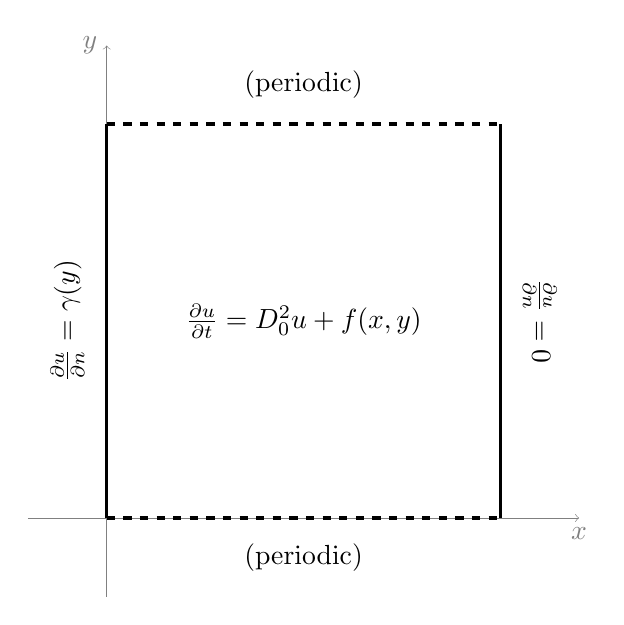
\begin{tikzpicture}[scale=5.0]
  \draw[->,gray,very thin] (-0.2,0.0) -- (1.2,0.0) node[below] {$x$};
  \draw[->,gray,very thin] (0.0,-0.2) -- (0.0,1.2) node[left] {$y$};
  \draw[line width=1.0pt] (0.0,0.0) -- (0.0,1.0);
  \draw[line width=1.0pt] (1.0,0.0) -- (1.0,1.0);
  \draw[line width=1.5pt,dashed] (0.0,0.0) -- (1.0,0.0);
  \draw[line width=1.5pt,dashed] (0.0,1.0) -- (1.0,1.0);
  \node at (0.5,0.5) {$\frac{\partial u}{\partial t} = D_0 \grad^2 u + f(x,y)$};
  \node at (0.5,-0.1) {(periodic)};
  \node at (0.5,1.1) {(periodic)};
  \node[rotate=90] at (-0.1,0.5) {$\frac{\partial u}{\partial n} = \gamma(y)$};
  \node[rotate=-90] at (1.1,0.5) {$\frac{\partial u}{\partial n} = 0$};
\end{tikzpicture}


\caption{Boundary conditions for a time-dependent heat equation problem.}
\label{fig:ts:heatsquare}
\end{figure}

In the interior we choose a particular formula for the source term,
    $$f(x,y) = 3 e^{-25(x-0.6)^2} \sin(2 \pi y).$$
Note that this takes both positive and negative values.  For the non-homogeneous boundary condition along the left side we have
	$$\frac{\partial u}{\partial n} = -\frac{\partial u}{\partial x} = \gamma(y),$$
where $n$ denotes the outward unit normal direction, with $\gamma(y) = \sin(6\pi y)$.  It is easy to verify (Exercise \ref{chap:ts}.\ref{exer:ts:zerototalsource}) that the totals of these particular sources are zero:
\begin{equation}
\int_{\mathcal{S}} f(x,y)\,dx\,dy = 0, \qquad \int_0^1 \gamma(y)\,dy = 0. \label{eq:ts:zerototalsource}
\end{equation}

Physically-speaking, total thermal (internal) energy is proportional to the integral of $u$ over $\mathcal{S}$.  (For a material with density $\rho$ and heat capacity $c$ the energy is $\rho c$ times the integral.)  On the other hand, equation \eqref{eq:ts:heatequation} is derived from the principle of conservation of energy \citep{Ockendonetal2003}.  Equation \eqref{eq:ts:heatequation} thus determines the evolution of total thermal energy, which is independent of time because of our particular choices:
\begin{align}
\frac{d}{dt} \left(\int_{\mathcal{S}} u(t,x,y)\,dx\,dy\right) &= D_0 \int_0^1 \gamma(y)\,dy + \int_{\mathcal{S}} f(x,y)\,dx\,dy \label{eq:ts:conservedscalar} \\
   &= 0. \notag
\end{align}
(See Exercise \ref{chap:ts}.\ref{exer:ts:zerototalsource}.)  We want our discretized version \eqref{eq:ts:molheat} to conserve energy too, so a feature of this example, shown below, is to add a energy ``monitor'' call-back to the \pTS object.


\section{Implementation}

The program \texttt{c/ch5/heat.c}, shown in Codes \ref{code:ts:heat:heatctx}--\ref{code:ts:heat:monitor} is straightforward to write based on our Chapter \ref{chap:st} and \ref{chap:nl} experience with \pDMDA.  It uses a \pTS object essentially as in the examples so far in this Chapter.  It has a simple context \texttt{struct} so that call-backs have access to the constant $D_0$ and functions $f$, $\gamma$ (Code \ref{code:ts:heat:heatctx}).

\cinputpart{heat.c}{\CODELOC}{A context \texttt{struct} gives call-backs access to constants and functions.}{I}{//HEATCTX}{//ENDHEATCTX}{code:ts:heat:heatctx}

In Code \ref{code:ts:heat:dmdasetup}, an extract of \texttt{main()}, we set up the grid \pDMDA object.  We specify periodicity in the $y$ direction so that, both in serial and in parallel, ghost points are available in the $y$ direction, below and above, respectively, the first and last ``real'' locations.

\cinputpart{heat.c}{\CODELOC}{Set up the \pDMDA grid object and allocate \pVecs for the solution $u$, heat source $f$, and Neumann boundary condition $\gamma$.}{II}{//DMDASETUP}{//ENDDMDASETUP}{code:ts:heat:dmdasetup}

The default grid of $m_x \times m_y = 5\times 4$ points, specified through arguments to \texttt{DMDACreate2d()} as shown in Code \ref{code:ts:heat:dmdasetup}, actually has square cells as shown in Figure \ref{fig:ts:heatdefaultgrid}.  In fact, the spacings of the grid are $1/(m_x-1)$ and $1/m_y$ respectively---see the helper function \texttt{Spacings()} in \texttt{heat.c} (not shown).  The grid points shown along the lower boundary $y=0$ in Figure \ref{fig:ts:heatdefaultgrid} are also ``present'' on the upper boundary $y=1$.

\begin{figure}
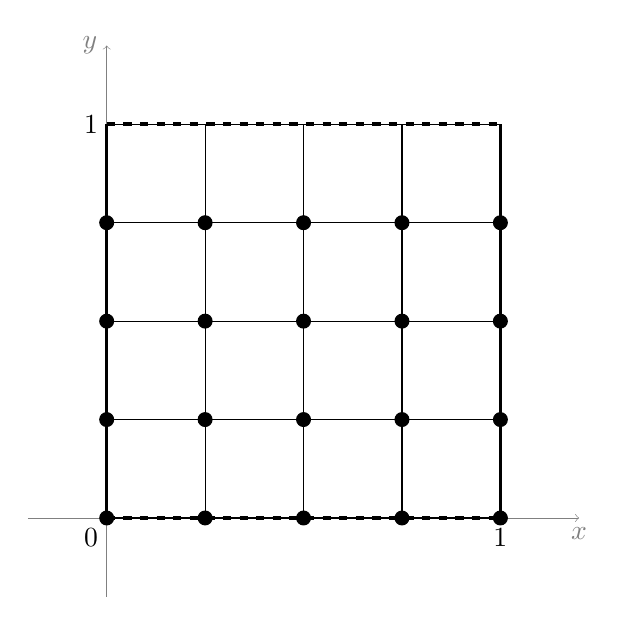
\begin{tikzpicture}[scale=5.0]
  \draw[->,gray,very thin] (-0.2,0.0) -- (1.2,0.0) node[below] {$x$};
  \draw[->,gray,very thin] (0.0,-0.2) -- (0.0,1.2) node[left] {$y$};
  \node at (-0.04,-0.05) {$0$};
  \node at (1.0,-0.05) {$1$};
  \node at (-0.04,1.0) {$1$};
  \pgfmathsetmacro\fourth{1.0/4.0}
  \draw[xstep=\fourth,ystep=\fourth,black,thin] (0.0,0.0) grid (1.0,1.0);
  \draw[line width=1.0pt] (0.0,0.0) -- (0.0,1.0);
  \draw[line width=1.0pt] (1.0,0.0) -- (1.0,1.0);
  \draw[line width=1.5pt,dashed] (0.0,0.0) -- (1.0,0.0);
  \draw[line width=1.5pt,dashed] (0.0,1.0) -- (1.0,1.0);
  \foreach \x in {0,...,4} {
    \foreach \y in {0,...,3} {
        \filldraw (\x * \fourth,\y * \fourth) circle (0.5pt);
    }
  }
\end{tikzpicture}


\caption{The default $5\times 4$ point grid for \texttt{heat.c} corresponds to square cells because of the periodicity in $y$.}
\label{fig:ts:heatdefaultgrid}
\end{figure}

Code \ref{code:ts:heat:dmdasetup} includes calls to \texttt{SetSource()} and \texttt{SetNeumanValues()} (not shown) to set $f,\gamma$ respectively.  A small idea here is that the non-homogeneous Neumann boundary value $\gamma(y)$ is allocated on a 2D grid even though it is only needed at points on the left boundary.  A slightly-less wasteful alternative, though requiring more code, would create a separate 1D \pDMDA for this boundary (Exercise \ref{chap:ts}.\ref{exer:ts:heatneumanndmda}).

\cinputpart{heat.c}{\CODELOC}{FIXME}{III}{//TSSETUP}{//ENDTSSETUP}{code:ts:heat:tssetup}

\cinputpart{heat.c}{\CODELOC}{FIXME}{II}{//RHSFUNCTION}{//ENDRHSFUNCTION}{code:ts:heat:rhsfunction}

\cinputpart{heat.c}{\CODELOC}{FIXME}{III}{//RHSJACOBIAN}{//ENDRHSJACOBIAN}{code:ts:heat:rhsjacobian}

\cinputpart{heat.c}{\CODELOC}{FIXME}{V}{//MONITOR}{//ENDMONITOR}{code:ts:heat:monitor}

\begin{figure}
% usage: \standardTSstack{scale}{Jacobian}{DMDA}
\standardTSstack{0.775}{}{}
\caption{The \PETSc stack used for the time-dependent, structured-grid PDE problems in Chapter \ref{chap:ts} (i.e.~\texttt{heat.c,pattern.c}).  Compare Figure \ref{fig:of:standardstack}.}
\label{fig:of:tsstack}
\end{figure}

FIXME

\begin{code}
run info
 $ ./heat -ts_view
 $ ./heat -ts_monitor -heat_monitor -snes_converged_reason

run-time graphics
 $ ./heat -da_refine 4 -ts_monitor -ts_monitor_solution draw -draw_pause 0.1
 $ mpiexec -n 4 ./heat -da_refine 1 -dm_view draw -draw_pause 2

good (use default BEULER):
 $ mpiexec -n 4 ./heat -ts_monitor -heat_monitor -snes_converged_reason -ts_monitor_solution draw -snes_monitor -da_refine 7

complete linear solve add -ksp_rtol 1.0e-12

explodes (as it should):
 $ ./heat -ts_monitor -ts_monitor_solution draw -da_refine 4 -ts_type rk -ts_adapt_type none

agonizingly slow (RK is adapting):
 $ ./heat -ts_monitor -ts_monitor_solution draw -da_refine 4 -ts_type rk

wobbles (typical Crank-Nicolson):
 $ ./heat -ts_monitor -ts_monitor_solution draw -da_refine 4 -ts_type cn

suppress wobbles by weighting implicitness more:
 $ ./heat -ts_monitor -ts_monitor_solution draw -da_refine 4 -ts_type theta -ts_theta_theta 0.6 -ts_theta_endpoint

better adaptive than rk:
 $ ./heat -ts_monitor -ts_monitor_solution draw -da_refine 4 -ts_type glle
\end{code}


\section{Coupled reaction-diffusion equations}

FIXME see pages 21--22 of \citep{HundsdorferVerwer2003} and see \citep{Pearson1993}

\cinputpart{pattern.c}{\CODELOC}{FIXME}{I}{//FIELDCTX}{//ENDFIELDCTX}{code:ts:pattern:fieldctx}

\cinputpart{pattern.c}{\CODELOC}{FIXME}{II}{//RHSFUNCTION}{//ENDRHSFUNCTION}{code:ts:pattern:rhsfunction}

\cinputpart{pattern.c}{\CODELOC}{FIXME}{III}{//IFUNCTION}{//ENDIFUNCTION}{code:ts:pattern:ifunction}

\cinputpart{pattern.c}{\CODELOC}{FIXME}{IV}{//IJACOBIAN}{//ENDIJACOBIAN}{code:ts:pattern:ijacobian}

\cinputpart{pattern.c}{\CODELOC}{FIXME}{V}{//TSSETUP}{//ENDTSSETUP}{code:ts:pattern:tssetup}

FIXME show use of \texttt{-ts\_type arkimex,theta}

FIXME final-time greyscale plots using \texttt{PetscBinaryIO.py}


\section{Exercises}

\renewcommand{\labelenumi}{\arabic{chapter}.\arabic{enumi}\quad}
\renewcommand{\labelenumii}{(\alph{enumii})}
\begin{enumerate}
\item \label{exer:ts:tan}  Consider the scalar ODE initial value problem $y'=1+y^2$, $y(0)=0$.  Show by-hand that $y(t)=\tan t$ is the (unique) solution.  Modify \texttt{ode.c} to solve this problem.  Run the code from $t_0=0$ to $t_f=2$.  What run-time evidence shows that your estimate of ``$y(2)$'' is totally meaningless?

\item \label{exer:ts:odepossible}  Which \pTS types work with \texttt{ode.c}, that is, do not give run-time errors?  Do \texttt{-help |grep ts\_type} to find possibilities, and try them.  Which ones work with the additional option \texttt{-snes\_fd}?  Which ones work with \texttt{odejac.c}?  Explain as much as you can.

\item \label{exer:ts:odeserial}  Code \texttt{ode.c} claims it is ``serial only.''  What happens with \texttt{mpiexec -n 2 ./ode}, and why?

\item \label{exer:ts:stiffexample}  Show by hand that the eigenvalues of matrix $B$ in \eqref{eq:ts:stiffexamplematrix} are $\lambda=i,-i,-101$.  Use a full eigen-decomposition $B = X \Lambda X^{-1}$, which can be computed by hand, to confirm \eqref{eq:ts:stiffsoln}, noting that
    $$e^{Bt} = X e^{\Lambda t} X^{-1} = X \begin{bmatrix} e^{\lambda_0 t} &  &  \\
                       & \ddots &  \\
                       & & e^{\lambda_{N-1} t} \end{bmatrix} X^{-1}.$$

\item \label{exer:ts:stiffcode}  Modify \texttt{odejac.c} to a similar code \texttt{stiff.c} which solves ODE IVP \eqref{eq:ts:stiffexample}.  It can use \texttt{VecView()} to print the computed solution and \texttt{TSGetTotalSteps()} for the number of steps.  Confirm the results shown in the text for \texttt{-ts\_type rk -ts\_rk\_type 2a} and for \texttt{-ts\_type cn}.

\item \label{exer:ts:stiffadaptive}  Continuing the above Exercise, use the default RK scheme RK3bs with adaptivity turned on, which is the default, but with an explicit accuracy goal set using options \texttt{-ts\_rtol}, \texttt{-ts\_atol}.  For example, run the following Bash loop:
\begin{code}
for POW in 2 3 4 5 6 7 8 9 10; do
    ./stiff -ts_type rk -ts_rtol 1.0e-$POW -ts_atol 1.0e-$POW
done
\end{code}
Conclude that for the Example problem on page \pageref{ex:ts:odestiff}, about 400 steps are necessary to get any accuracy at all (i.e.~at least one digit) using method RK3bs.

\item \label{exer:ts:absstabcases}  Confirm formulas \eqref{eq:ts:absstabcases}.  Sketch the regions of absolute stability shown in Figure \ref{fig:ts:absstabregions} and locate the $z$-values corresponding to the runs shown in Figure \ref{fig:ts:absstabfail}.

\item \label{exer:ts:stiffdecayasymptotic}  Show that \eqref{eq:ts:stiffdecaytestproblem} has solution
    $$y(t) = e^{\lambda t} - \lambda \int_0^t e^{\lambda (t-s)} \gamma(s)\,ds.$$
Then show that the family of functions $D_\lambda(x) = -\lambda e^{\lambda x}$ form a Dirac delta function \citep{Evans2010} in the sense that, for any continuous function $\varphi(x)$, $\int_{0}^\infty D_\lambda(x) \varphi(x)\,dx = \varphi(0)$ as $\Re\lambda \to -\infty$.  Conclude that the solution to \eqref{eq:ts:stiffdecaytestproblem} is asymptotic to $\gamma(t)$ as $\Re\lambda \to -\infty$.

\item \label{exer:ts:fdjacobian}   Adding option \texttt{-snes\_monitor} so a to look deeper, the results of these three runs
\begin{cline}
$ ./ode -ts_type cn -snes_fd -snes_monitor
$ ./ode -ts_type cn -snes_mf -snes_monitor
$ ./odejac -snes_monitor
\end{cline}
%$
differ in the size of residual norms and even in the number of Newton iterations.  Explain.

\item \label{exer:ts:zerototalsource}  Show \eqref{eq:ts:zerototalsource}.  Then fill in the details to show \eqref{eq:ts:conservedscalar}.  Observe that the periodic boundary condition amounts to treating the top/bottom boundary locations as interior points of a (topologically) cylindrical surface.

\item \label{exer:ts:heatneumanndmda} Write a new version of \texttt{heat.c} which creates a \texttt{DMDACreate1d()} and uses it to allocate and access the \pVec \texttt{gamma}.  The new code will not waste memory in a 2D array for this purpose, as does \texttt{heat.c}.

\item FIXME for run like
\begin{cline}
./pattern -da_refine 6 -ptn_tf 500 -ptn_steps 100 -ts_monitor -snes_converged_reason
\end{cline}
which is fastest among these nine ARKIMEX and three $\theta$ methods?:
\begin{code}
-ts_type arkimex -ts_arkimex_type [a2|l2|ars122|2c|2d|2e|3|4|5]
-ts_type theta -ts_theta_endpoint -ts_theta_theta [0.5|0.75|1]
\end{code}
Are any other adaptive \pTS types faster?  Also compare final frames from \texttt{-ts\_monitor\_solution draw}; how worried should we be about the effect of time-stepping on the solution of this problem?

\end{enumerate}
